\chapter{Statistical Analysis}
\label{chap:Results}

%%%%%%%%%%%%%%%%%%%%%%%%%%%%%%%%%%%%%%%%%%%%%%%%%%%%%%%%%%%
%%%%%%%%%%%%%%%%%%%%%%%%%%%%%%%%%%%%%%%%%%%%%%%%%%%%%%%%%%%

\section{Profile Likelihood Fit}
\label{sec:PLF}

A binned likelihood function $\mathcal{L}(\mu, \theta)$ is constructed to perform the statistical analysis on the BDT discriminator distributions. The parameter of interest (POI), denoted by $\mu$, is the signal strength that governs the cross section of the top decay and production signals simultaneously. All the uncertainties are incorporated into the likelihood function as nuisance parameters, denoted by $\theta$. The uncertainties that affect the shape of the BDT discriminator distributions are considered with Gaussian distributions while other uncertainties that only affect the normalizations are considered with log-normal distributions. 

To control the systematic uncertainties, a profile likelihood fit is performed simultaneously in six regions (three data-taking years and two \acp{SR}) by maximizing the likelihood function $\mathcal{L}(\hat{\mu}, \hat{\theta})$. Both $\hat{\mu}$ and $\hat{\theta}$ are the maximum likelihood estimators for the signal strength and nuisance parameters, respectively. The post-fit distributions of the BDT discriminator are shown in Fig.~\ref{fig:bdt_postfit_VecU}. The most prominent uncertainties affecting the likelihood fit are the statistical uncertainties that arise from limited sample size.

\begin{figure}[tbh!]
 \begin{center}
 \begin{tabular}{cc}
  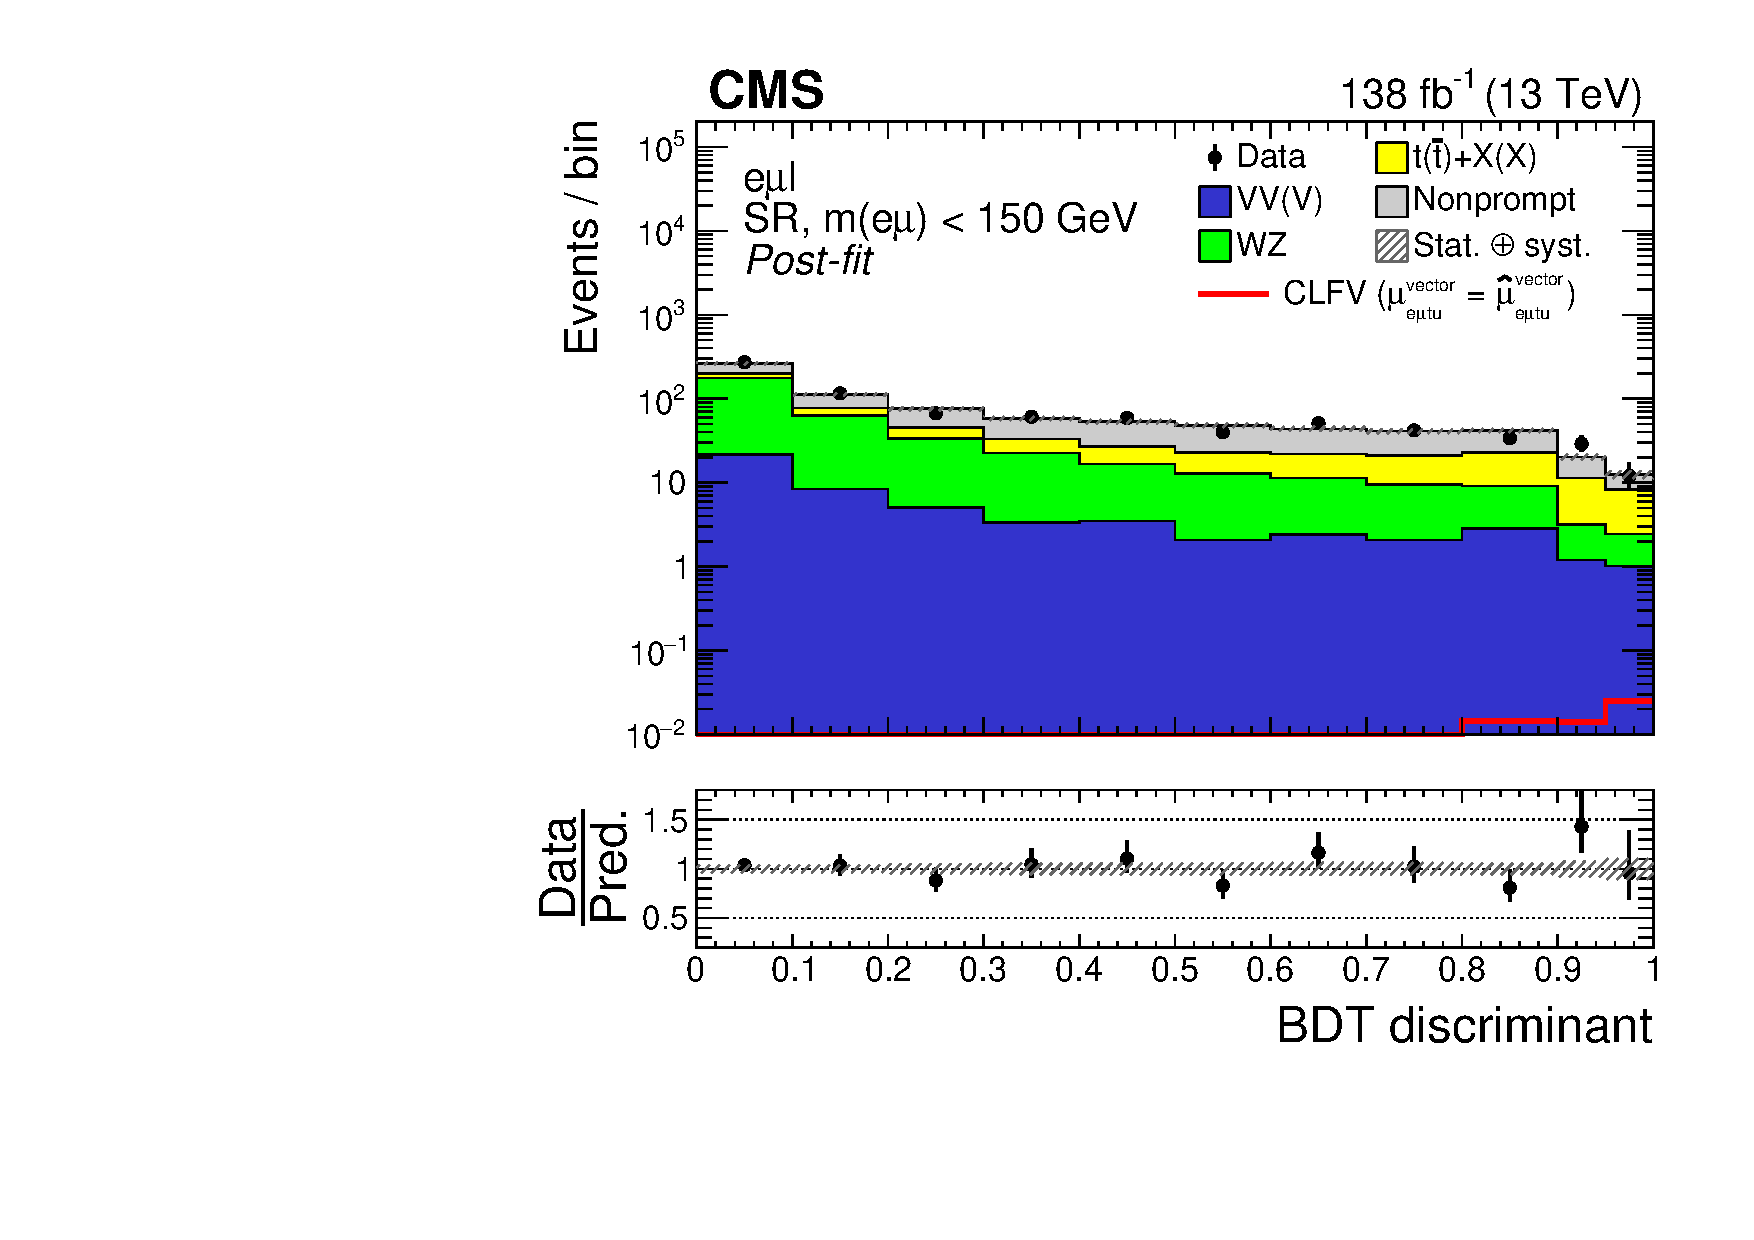
\includegraphics[width=0.48\textwidth]{figures/Part3/Results/BDT_TT_VecU}&
  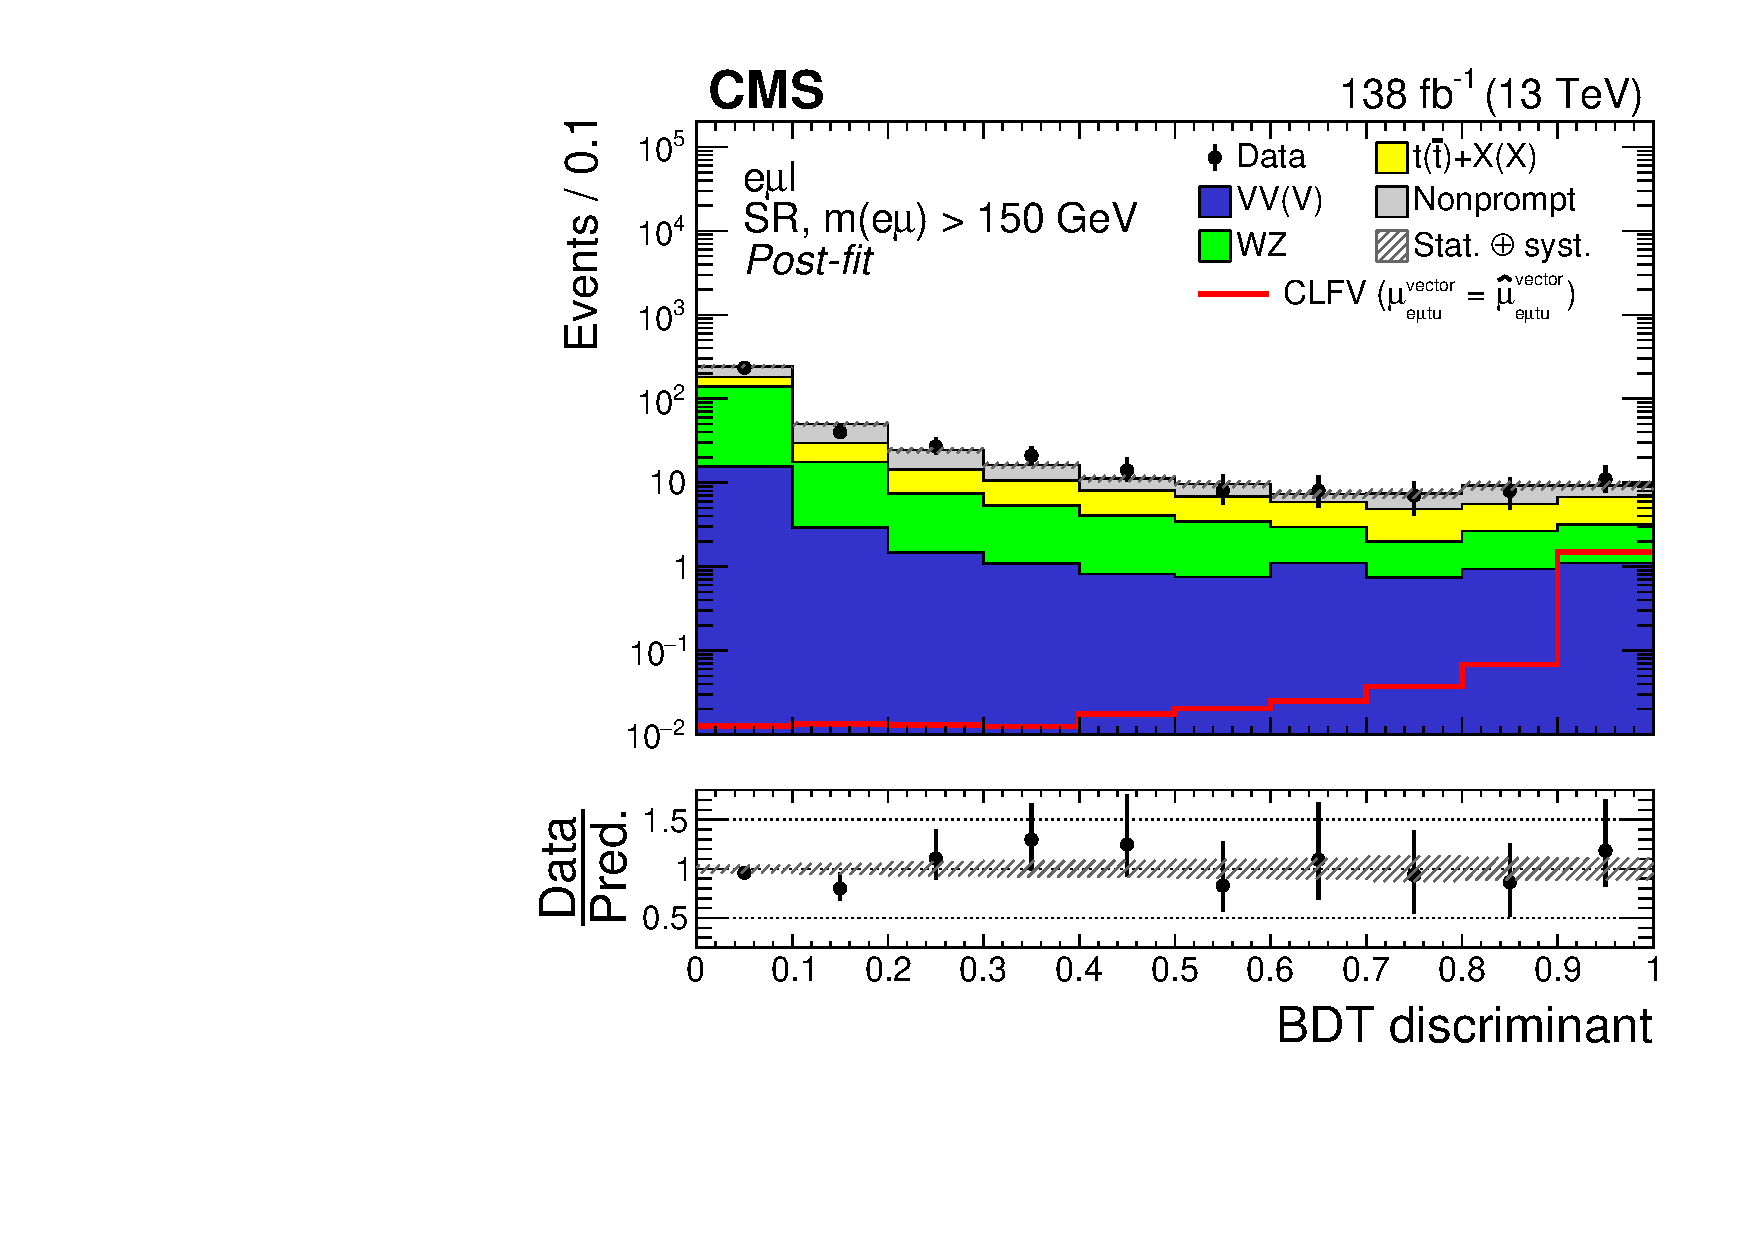
\includegraphics[width=0.48\textwidth]{figures/Part3/Results/BDT_ST_VecU}\\
 \end{tabular}
 \caption{Distributions of the post-fit BDT discriminator targeting the CLFV top quark decay (left) and production (right) signal. Contributions from the two signal modes (production and decay) are combined within each SR and are shown as the solid red line. The post-fit signal strength ($\mu_{\emut{u}}^{\textsf{vector}}=\hat{\mu}_{\emut{u}}^{\textsf{vector}}$) is used to normalise the signal cross sections. The hatched bands indicate post-fit uncertainties (statistical and systematic) for the SM background predictions.}
 \label{fig:bdt_postfit_VecU}
 \end{center}
\end{figure} 
%%%%%%%%%%%%%%%%%%%%%%%%%%%%%%%%%%%%%%%%%%%%%%%%%%%%%%%%%%%
%%%%%%%%%%%%%%%%%%%%%%%%%%%%%%%%%%%%%%%%%%%%%%%%%%%%%%%%%%%

\section{Upper Limits}
\label{sec:Limits}

The results for the one-dimensional limits are summarized in Table~\ref{tab:limit}. Assuming a linear relationship between $\mathcal{B}(\tto{c})$ and $\mathcal{B}(\tto{c})$ in the case of nonvanishing signals, the two-dimensional limits can also be obtained through interpolation (see Fig.~\ref{fig:2dlimit}). This analysis constitutes the most stringent limits on these processes to date.

\begin{table}[th]
\sffamily
\centering
\caption{Upper limits at 95\% CL on Wilson coefficients and the branching fractions. The expected and observed upper limits are shown in regular and bold fonts, respectively. The intervals that contain 68\% of the distribution of the expected upper limits are shown in parentheses.}
\resizebox{0.95\linewidth}{!}{%
\begin{tabular}{cccccc}
\toprule
CLFV  & Lorentz  & \multicolumn{2}{c}{$\WC{}{\emut{q}}/\mathrm{\Lam}^2~(\TeV^{-2})$} & \multicolumn{2}{c}{$\mathcal{B} (\tto{q}) \times 10^{-6}$} \\
coupling  & structure & exp (68\% range) & obs & exp (68\% range) & obs \\
\midrule
\multirow{3}{*}{$\emut{u}$}& tensor  & 0.022 (0.018--0.026) & \textbf{0.024} & 0.027 (0.018--0.040) & \textbf{0.032}\\
& vector & 0.044 (0.036--0.054) & \textbf{0.048} & 0.019 (0.013--0.028) & \textbf{0.022}\\
& scalar & 0.093 (0.077--0.114) & \textbf{0.101} & 0.010 (0.007--0.016) & \textbf{0.012}\\
\midrule
\multirow{3}{*}{$\emut{c}$} & tensor & 0.084 (0.069--0.102) & \textbf{0.094} & 0.396 (0.272--0.585) & \textbf{0.498}\\
 & vector & 0.175 (0.145--0.214) & \textbf{0.196} & 0.296 (0.203--0.440) & \textbf{0.369}\\
 & scalar & 0.385 (0.318--0.471) & \textbf{0.424} & 0.178 (0.122--0.266) & \textbf{0.216}\\
 \bottomrule
\end{tabular}
}
\label{tab:limit}
\end{table}

\begin{figure}[tbh!]
 \begin{center}
 \begin{tabular}{cc}
  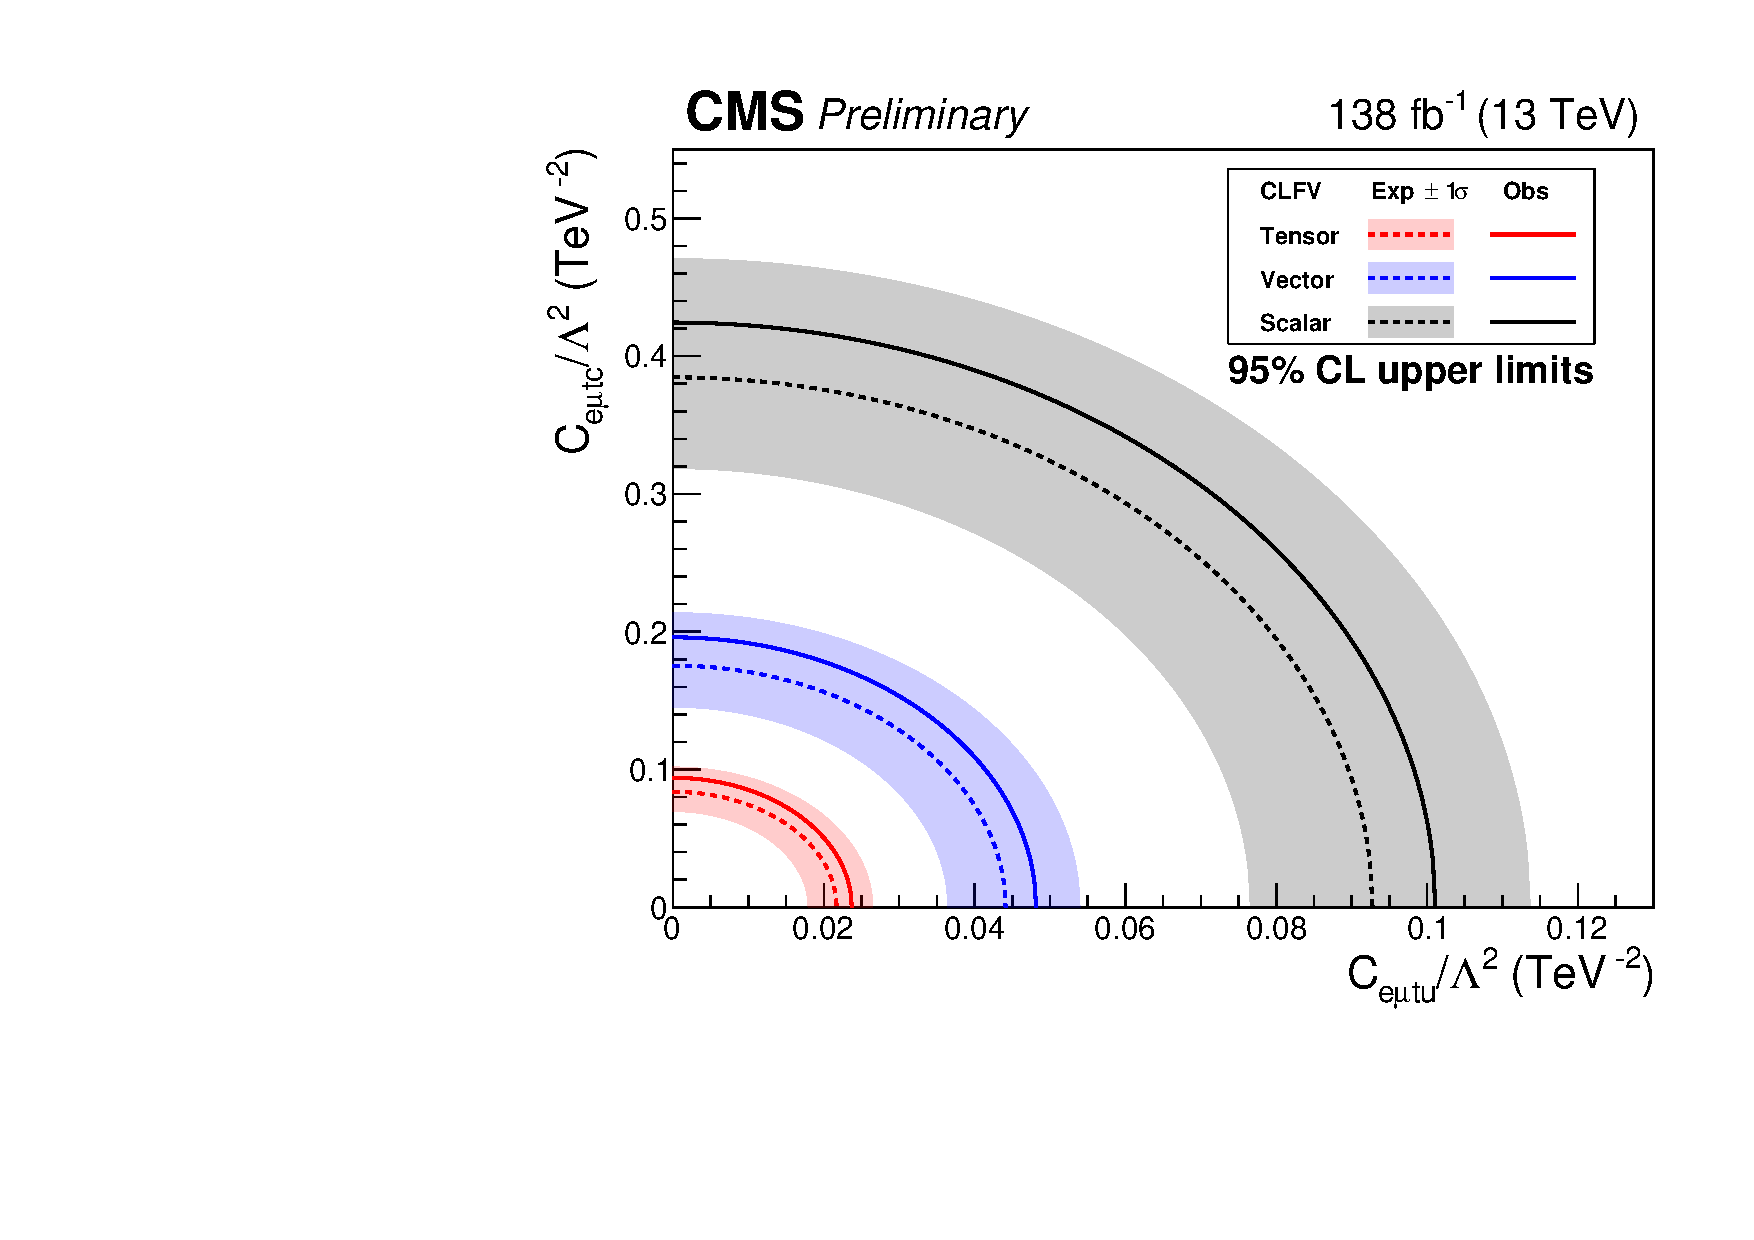
\includegraphics[width=0.48\textwidth]{figures/Part3/Results/Hist2D_WC}&
  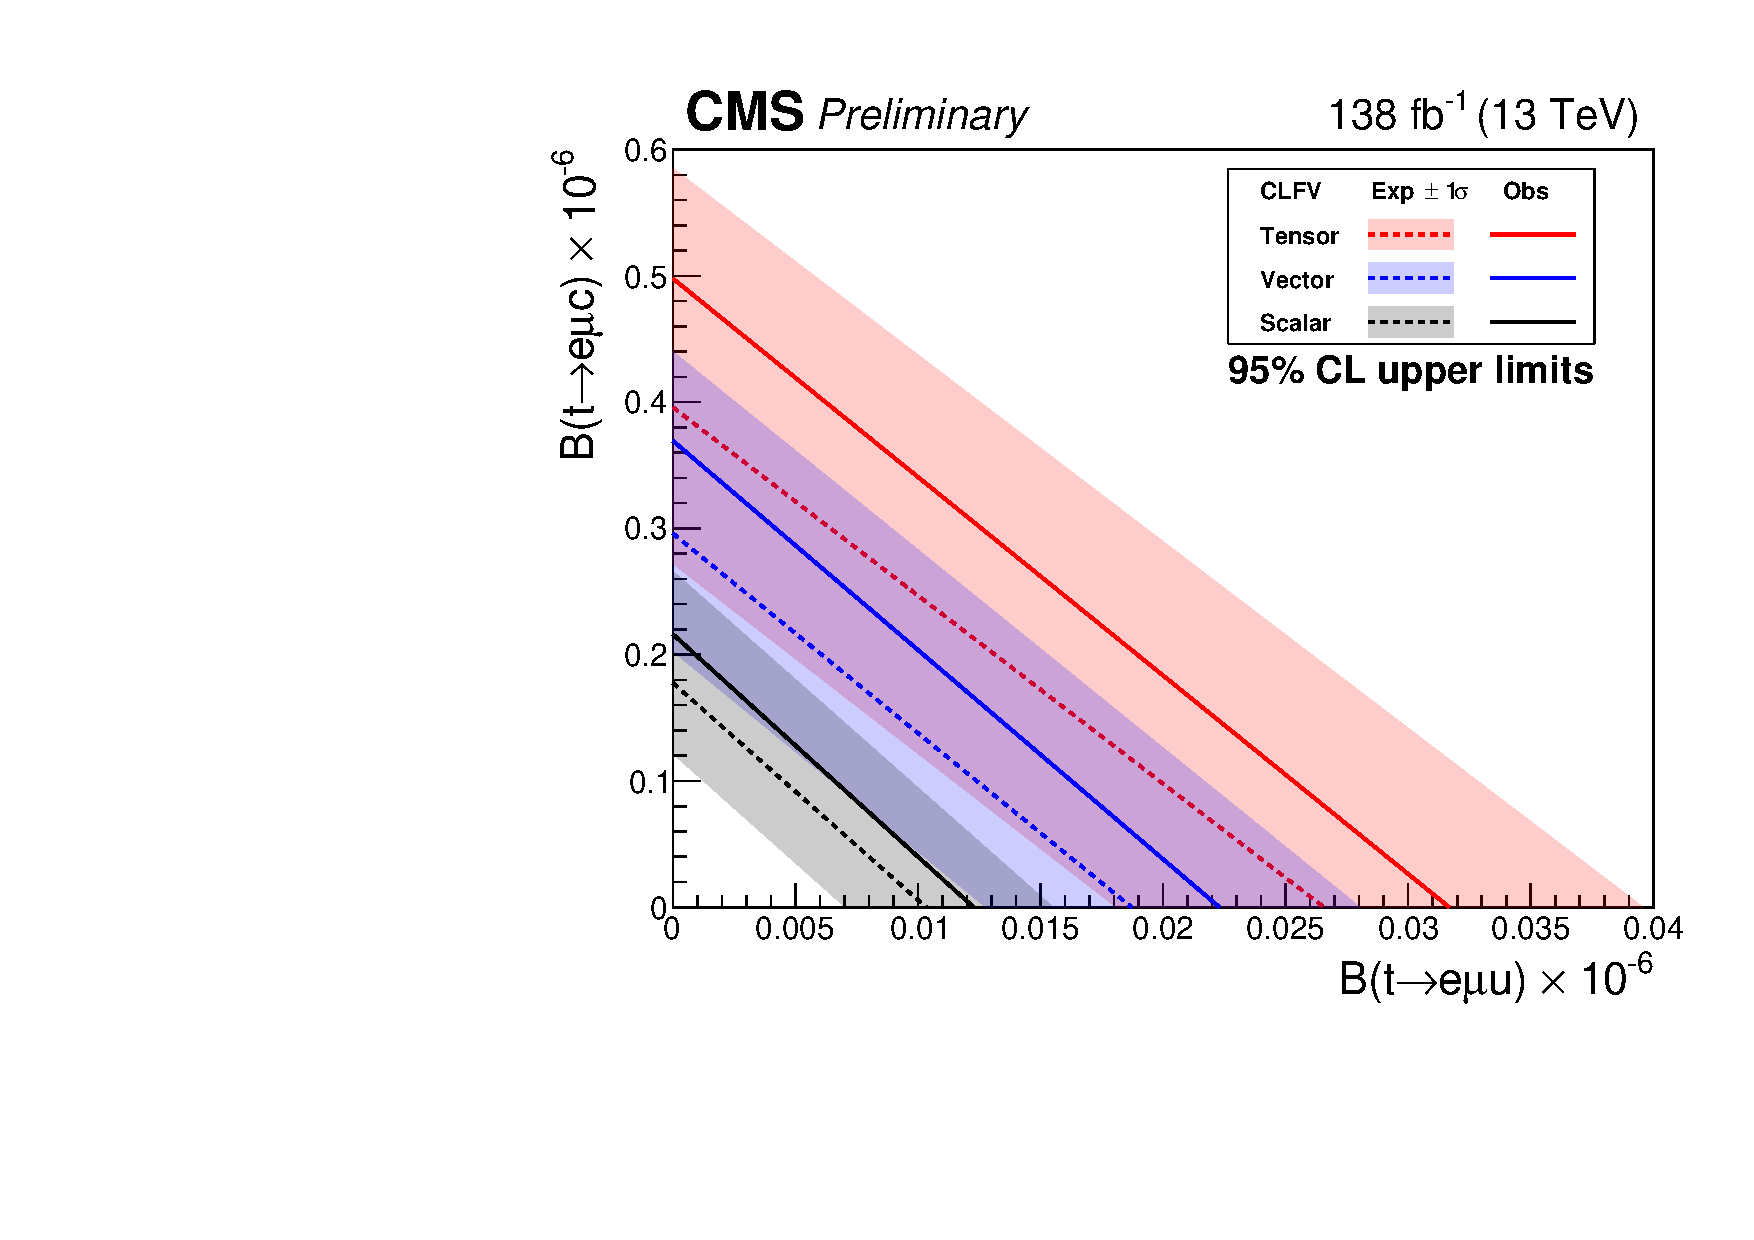
\includegraphics[width=0.48\textwidth]{figures/Part3/Results/Hist2D_BR}\\
 \end{tabular}
 \caption{Two-dimensional 95$\%$ CL upper limits on the Wilson coefficients (left) and the branching fractions (right). The observed (expected) upper limits for tensor-, vector-, and scalar-like CLFV interactions are shown in red, blue, and black solid (dotted) lines, respectively. The shaded bands contain $68\%$ of the distribution of the expected upper limits.}
 \label{fig:2dlimit}
 \end{center}
\end{figure}